%=====================================================================
%  MODELO DE ARTÍCULO / MONOGRAFÍA — MECÁNICA CUÁNTICA
%  Plantilla elegante en LaTeX  ·  compílese con pdfLaTeX
%  Secuencia:  pdflatex → bibtex → pdflatex → pdflatex
%---------------------------------------------------------------------
%  Autor de la plantilla: (adáptese libremente)
%  Diseño: paleta cálida "Navajo" · tipografía Palatino (mathpazo)
%=====================================================================

\documentclass[11pt,letterpaper]{article}

%========================  CODIFICACIÓN E IDIOMA  =====================
\usepackage[T1]{fontenc}
\usepackage[utf8]{inputenc}
\usepackage{babel}
\babelprovide[import,main]{spanish}          % locale español (babel moderno)

%========================  MATEMÁTICAS Y FUENTE  =====================
\usepackage{amsmath,amssymb}
\usepackage{bm}
\usepackage[sc]{mathpazo}     % Palatino: elegante y muy legible en física
\linespread{1.05}             % interlineado ligeramente holgado
\usepackage{microtype}        % micro-tipografía: mejor gris de página

%========================  GEOMETRÍA Y FIGURAS  ======================
\usepackage[letterpaper,left=2.0cm,right=2.0cm,top=2.0cm,bottom=2.0cm]{geometry}
\usepackage{graphicx}
\usepackage{float}
\usepackage{booktabs}         % reglas de tabla profesionales

%========================  PALETA DE COLOR (navajo_seq)  =============
\usepackage{xcolor}
% Diez tonos del colormap secuencial navajo_seq (frío -> cálido):
\definecolor{navaMidnight}{HTML}{0D1B2A}  % azul noche
\definecolor{navaDeep}{HTML}{1B3A4B}      % pizarra profunda
\definecolor{navaBlue}{HTML}{2E6E8E}      % azul-petróleo
\definecolor{navaTurq}{HTML}{4FA8B8}      % turquesa
\definecolor{navaAqua}{HTML}{88C9C8}      % aguamarina claro
\definecolor{navaCream}{HTML}{F2E8D0}     % crema
\definecolor{navaSand}{HTML}{E8A87C}      % arena / terracota clara
\definecolor{navaBurnt}{HTML}{C46D3B}     % naranja quemado
\definecolor{navaBrick}{HTML}{A0372A}     % ladrillo
\definecolor{navaMaroon}{HTML}{6B1E1E}    % granate oscuro
% Roles del documento (cálidos = jerarquía; frío = enlaces externos):
\colorlet{siena}{navaMaroon}     % títulos de sección, etiqueta Resumen, pies
\colorlet{terracota}{navaBrick}  % subsecciones, enlaces internos, recuadros
\colorlet{ocre}{navaBurnt}       % reglas de acento (portada y secciones)
\colorlet{turquesa}{navaBlue}    % citas y URLs
\colorlet{adobe}{navaSand}       % filetes suaves del resumen
\colorlet{crema}{navaCream}      % fondos de recuadro

%========================  TÍTULOS DE SECCIÓN  =======================
\usepackage{titlesec}
\titleformat{\section}[hang]
  {\normalfont\large\bfseries\color{navaDeep}}
  {\thesection}{0.7em}{}
  [{\vspace{2pt}\color{ocre}\titlerule[0.8pt]}]
\titleformat{\subsection}[hang]
  {\normalfont\normalsize\bfseries\color{navaBlue}}
  {\thesubsection}{0.6em}{}
\titlespacing*{\section}{0pt}{1.6em}{0.7em}
\titlespacing*{\subsection}{0pt}{1.1em}{0.4em}

%========================  PIES DE FIGURA / TABLA  ===================
\usepackage{caption}
\captionsetup{font=small,labelsep=period,labelfont={bf,color=siena}}

%========================  BIBLIOGRAFÍA (natbib)  ====================
\usepackage[numbers,sort&compress]{natbib}
\bibpunct{[}{]}{,}{n}{}{,}

%========================  RECUADROS DE CONSEJO  =====================
\usepackage[most]{tcolorbox}
\newtcolorbox{consejo}{
  enhanced, breakable,
  colback=crema, colframe=terracota,
  boxrule=0.4pt, arc=2.5pt, outer arc=2.5pt,
  left=10pt, right=10pt, top=8pt, bottom=8pt,
  fontupper=\small,
  coltitle=white, colbacktitle=terracota,
  fonttitle=\bfseries\small,
  title=Consejo de redacción,
  attach boxed title to top left={xshift=10pt, yshift=-\tcboxedtitleheight/2},
  boxed title style={boxrule=0pt, arc=2pt},
  top=12pt
}

%========================  OPERADORES Y ATAJOS  ======================
\DeclareMathOperator{\sech}{sech}
\newcommand{\ii}{\mathrm{i}}          % unidad imaginaria
\newcommand{\dd}{\mathrm{d}}          % diferencial recto
\newcommand{\vc}[1]{\bm{#1}}          % vectores en negrita
\newcommand{\op}[1]{\hat{#1}}         % operadores con sombrero

%========================  HIPERVÍNCULOS  ============================
\usepackage[unicode=true,pdfusetitle,colorlinks=true,
            bookmarks=true,pdfborder={0 0 0}]{hyperref}
\hypersetup{linkcolor=terracota, citecolor=turquesa, urlcolor=turquesa}

%---------------------------------------------------------------------
%  Datos del trabajo
%---------------------------------------------------------------------
\newcommand{\subtitulo}{Subtítulo opcional del trabajo}
\title{Título del trabajo}
\author{Nombre del Estudiante}
\date{\today}

\begin{document}

%=====================================================================
%  PORTADA
%=====================================================================
\begin{center}
  {\color{ocre}\rule{0.5\textwidth}{0.8pt}}\\[1.1em]
  {\LARGE\bfseries\color{navaMidnight} Desigualdades de Bell y entrelazamiento atómico}\\[0.45em]
  %{\large\itshape \subtitulo}\\[1.2em]
  {\scshape\large Juan Alexis Hernández Hernández}\\[0.35em]
  {\small Curso de Introducción a la Física Atómica y Molecular\ \textperiodcentered\ Facultad de Ciencias, UNAM\\
   \texttt{alexi5@ciencias.unam.mx}}\\[0.5em]
  {\small \today}\\[0.6em]
  {\color{ocre}\rule{0.5\textwidth}{0.8pt}}
\end{center}
\vspace{0.6em}

%=====================================================================
%  RESUMEN
%=====================================================================
\begin{center}
\begin{minipage}{0.88\textwidth}
  {\color{adobe}\rule{\linewidth}{0.6pt}}\par\vspace{0.6em}
  \small
  \noindent{\bfseries\color{siena} Resumen.\ }%
  	En este trabajo se estudió la relación entre la paradoja EPR, las desigualdades de Bell y el entrelazamiento cuántico. Partiendo de un sistema de dos partículas de espín $\frac{1}{2}$ preparadas en el estado singlete, se retomó el argumento EPR sobre la completitud de la Mecánica Cuántica. Posteriormente, mediante un enfoque gráfico basado en las suposiciones de realismo local y las anticorrelaciones perfectas del estado singlete, se realizó una deducción de la desigualdad original de Bell. Al comparar esta desigualdad con las correlaciones predichas por la Mecánica Cuántica, se encontró que existen direcciones de medición para las cuales es violada. Este resultado muestra que las correlaciones cuánticas estudiadas no pueden ser reproducidas por una teoría de variables ocultas locales bajo las suposiciones consideradas, permitiendo relacionar este resultado con el estudio del entrelazamiento en sistemas atómicos de dos niveles.
  
  \par\vspace{0.7em}
  \noindent{\footnotesize\itshape Palabras clave:\/} paradoja EPR, desigualdades de Bell, entrelazamiento cuántico, estado singlete, realismo local. %ejemplo, plantilla, mecánica cuántica.
  \par\vspace{0.6em}
  {\color{adobe}\rule{\linewidth}{0.6pt}}
\end{minipage}
\end{center}
\vspace{1.2em}

%=====================================================================
%  INTRODUCCIÓN
%=====================================================================
\section{Introducción}\label{sec:introduccion}
En 1935, Albert Einstein, Boris Podolsky y Nathan Rosen (EPR) hicieron manifiesto de su postura sobre la teoría de la Mecánica Cuántica. Ellos sugieren que la descripción cuántico-mecánica de la realidad dada por las funciones de onda no es completadejando abierta la pregunta sobre si existe o no tal descripción que hagan de la mecánica cuántica una teoría completa. \cite{EPR} Este artículo, a pesar de sí tener una parte matemática, llega a rozar lo "filosófico" sobre lo que implica y lo que no implica la teoría de la Mecánica Cuántica, introduciendo un concepto (no exahustivo) sobre lo que implica que algo sea "real".

En 1964, John Bell, con estos dos desarrollos (más algunos varios más) en el primer volumen de la revista Pyhsics, formula lo que ahora se conocen como la desigualdad de Bell. Es la formulación matemática que se debe de satisfacer si un sistema es local y real. 

Años más tarde, numerosos autores deducen variantes de esta desigualdad, sin embargo, la suposición de un realismo local no se presenta como un paso lógico específico para derivar las desigualdades. Es por ello que en este trabajo, no sin antes enunciar una forma de la "paradoja" EPR, se retomará el caso de un estado entrelazado de dos partículas y se hará una deducción de la desigualdad original de Bell sin pasar por una teoría de variables ocultas de manera explícita, y apoyándose de un método gráfico realizado por Krzysztof Rebilas \cite{Rebilas} para desarrollarlo de una manera más intuitiva. Finalmente, se abordará qué implicaciones tiene que no se cumpla esa desigualdad que planteó Bell bajo estas hipótesis.


%=====================================================================
%  DESARROLLO Y MÉTODOS
%=====================================================================
\section{Desarrollo y métodos}\label{sec:desarrollo}
\subsection{EPR}%\label{subsec:dinamica}

EPR pone en discusión dos preguntas:
\begin{gather}
	\text{¿La teoría de la Mecánica Cuántica es correcta?}
	\label{qst:es_correcta}
	\\
	\text{¿Es completa la descripción que da la teoría de la Mecánica Cuántica?}
	\label{qst:completitud}
\end{gather}

entendiendo que "completa" es que: cada elemento de la realidad debe de tener una contraparte en la teoría física. \cite{EPR}

Ellos ponen en mesa que la corrección de una teoría se juzga por el grado de concordancia entre las conclusiones de esa teoría y la experiencia humana; en la física, esa experiencia humana toma la forma de experimento y medición. Es así como en lugar de tratar de ver si es correcta o no la Mecánica Cuántica (responder \ref{qst:es_correcta}), se discutió sobre si se respeta la completitud de esa teoría (\ref{qst:completitud}).

Por otro lado, definieron como "realidad" a aquello que: si, sin perturbar en absoluto el sistema, podemos predecir con certeza (i.e., probabilidad igual a $1$) el valor de una magnitud física, entonces existe un elemento de la realidad física correspondiente a esta magnitud física. \cite{EPR}

Y es así como tras pequeña descripción matemática con el uso de operadores (observables) de posición y momento, y una función de onda de dos partículas, demostraron que o
\begin{equation}
	\text{\parbox{0.85\linewidth}{\centering la descripción de la mecánica cuántica de la realidad dada por la función de onda no es completa}}
	\label{qst:incompletitud}
\end{equation}
o bien
\begin{equation}
	\text{\parbox{0.85\linewidth}{\centering cuando los operadores correspondientes a dos magnitudes físicas no conmutan, las dos magnitudes no pueden tener realidad simultánea. \cite{EPR}}}
	\label{qst:no_real_simul}
\end{equation}
Entonces, partiendo de la suposición de que la función de onda sí proporciona una descripción completa de la realidad física, se llega a la conclusión de que dos cantidades físicas, con operadores que no conmutan, pueden tener una realidad simultánea; por tanto, la negación de \ref{qst:incompletitud} lleva a la negación de la única otra alternativa, \ref{qst:no_real_simul}.

Dado que la demostración original en EPR de esto último contempla variables continuas, recuperemos una reformulación de este experimento que contempla variables discretas \cite{Apuntes}: el espín en un estado singlete, ya que es como lo manejó Bell (que discutiremos más adelante):

Consideremos un sistema de dos partículas de espín $\frac{1}{2}$, preparadas inicialmente en un estado entrelazado en particular: el estado singlete

$$ |\psi\rangle_{12} = \frac{1}{\sqrt{2}} ( |\uparrow_z\rangle_1 |\downarrow_z\rangle_2 - |\downarrow_z\rangle_1 |\uparrow_z\rangle_2 ), $$
las partículas se separan espacialmente, de modo que la partícula 1 es enviada a Alice y la partícula 2 a Bob.

\textbf{(i)} Alice elige medir una componente del espín de su partícula, por ejemplo $S_z^{(1)}$.
\begin{gather*}
	\text{Si la medición de Alice resulta en } S_z^{(1)} = +\frac{\hbar}{2} \Rightarrow \text{el estado de Bob es } |\downarrow_z\rangle_2
	\\
	\text{y si Alice mide } S_z^{(1)} = -\frac{\hbar}{2} \Rightarrow \text{el estado de Bob es } |\uparrow_z\rangle_2.
\end{gather*}

\textbf{(ii)} Alternativamente, Alice puede elegir medir otra componente, por ejemplo $S_x^{(1)}$.
\begin{gather*}
	\text{Si la medición de Alice resulta en } S_x^{(1)} = +\frac{\hbar}{2} \Rightarrow \text{el estado de Bob es } |\downarrow_x\rangle_2
	\\
	\text{y si Alice mide } S_x^{(1)} = -\frac{\hbar}{2} \Rightarrow \text{el estado de Bob es } |\uparrow_x\rangle_2.
\end{gather*}

\textbf{(iii)} Sin embargo, los operadores correspondientes a las componentes $x$ y $z$ del espín de Bob no conmutan:
\begin{equation}
	[S_x^{(2)},S_z^{(2)}] = -i\hbar S_y^{(2)} \neq 0
	\label{eq:contradiccion}
\end{equation}

Por lo tanto, bajo el criterio de realidad de EPR, y suponiendo que la medición realizada por Alice no perturba físicamente a la partícula de Bob, ambas componentes del espín deberían corresponder a elementos de realidad física, pues Alice puede elegir cuál predecir con certeza. Sin embargo, la Mecánica Cuántica no permite representarlas simultáneamente mediante valores definidos en un mismo estado cuántico.  \cite{Apuntes} Por ello, EPR concluye que la descripción proporcionada por la función de onda es incompleta. \cite{EPR}
%
%
%
%
\subsection{Desigualdades de Bell}%\label{subsec:dinamica}
J. Bell, en 1964, demostró que cualquier teoría que trate las partículas bajo la suposición del "realismo local" es incompatible con las predicciones de la Mecánica Cuántica. Recuperemos el enfoque gráfico de la deducción de las desigualdades de Bell de Krzystof Reblias, ya que la demostración origial utiliza la premisa de realismo local como una estructura matemática específica en lugar de un paso lógico en la derivación, lo que puede ser dificíl de entender. \cite{Rebilas}

Primero, tomemos en cuenta que la combinación de las siguientes asunciones es lo que denominaremos como realismo local: se considera que ciertas partículas poseen ciertas propiedades, descritas por la llamada "variable oculta" $\lambda$, que determinan de manera única los resultados $A$ y $B$, independiente de qué medición se realice realmente. Mientras, la asunción del localismo significa que el resultado de $A$ logrado por Alice no depende de los ajustes de medición elegidos por Bob entre las dos posibilidades, $\{b, b'\}$, y de manera similar, el resultado $B$ obtenido por Bob no está influenciado por los ajustes del aparato de Alice, $\{a, a'\}$. \cite{Rebilas}

Consideremos nuevamente un experimento con dos partículas entrelazadas, donde Alice puede elegir entre dos direcciones de medición, $a$ y $c$, mientras que Bob puede elegir entre $b$ y $c$, y los resultados posibles de sus mediciones serán $A=\pm1$ y $B=\pm1$, respectivamente.

De la suposición de localidad, se sigue que para el mismo par exacto de partículas
\begin{gather*}
	A(a,b)=A(a,c)=A(a),
	\\
	B(b,a)=B(b,c)=B(b).
\end{gather*}
donde $A(a,b)$ denota el resultado $A$ que sería registrado por Alice si su configuración fuera $a$ mientras que la de Bob es $b$. Análogamente con $B(b,a)$. Ahora bien, dado que estamos considerando partículas en el estado singlete, sabemos que sus resultados son perfectamente opuestos cuando Alice y Bob miden en la misma dirección. Por lo tanto,
$$ A(c)=-B(c), $$
lo que implica que no puede existir un par de partículas para el cual ambos obtengan $-1$ al medir en la dirección $c$.

Bajo estas suposiciones, para cada par de partículas podemos asignar resultados a las cuatro combinaciones posibles de direcciones, aun cuando solamente una de ellas sea medida experimentalmente. Esta es la idea detrás de la representación gráfica de Rębilas: cada par de partículas queda representado por un rectángulo cuyos cuatro vértices son los que corresponden a los resultados que se obtendrían para las diferentes elecciones de medición.

\begin{figure}%[H]
	\centering
	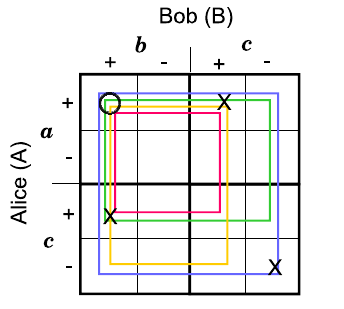
\includegraphics[scale=01]{figs/grafica.png}
	\caption{Las configuraciones de medición y las cajas marcadas con X para las derivaciones de la desigualdad de Bell. \cite{Rebilas}}
	\label{fig:graf}
\end{figure}

Utilizando la representación de la Figura \ref{fig:graf}, consideremos el conjunto de pares de partículas que producirían los resultados $A(a)=+1$ y $B(b)=+1$, que denotaremos por $\{a^+,b^+\}$. Como se observa en la gráfica, cualquier par que pertenezca a este conjunto necesariamente debe pertenecer también a alguno de los conjuntos $\{a^+,c^+\}$ o $\{c^+,b^+\}$. Esto se debe a que la posibilidad $\{c^-,c^-\}$ está excluida por la anticorrelación del estado singlete.

Si $n(a^+,b^+)$ representa el número de pares que producirían los resultados $\{a^+,b^+\}$, entonces no es mayor que la suma de los números pares de los conjuntos mencionados anteriormente
\begin{equation}
	n(a^+,b^+) \leq n(a^+,c^+) + n(c^+,b^+).
	\label{eq:des_1}
\end{equation}

De manera análoga, si intercambiamos los signos de los resultados, obtenemos
\begin{equation}
	n(a^-,b^-) \leq n(a^-,c^-) + n(c^-,b^-).
	\label{eq:des_2}
\end{equation}

Sumando las Ecuaciones \ref{eq:des_1} y \ref{eq:des_2},
\begin{equation}
	n(a^+,b^+)+n(a^-,b^-)
	\leq n(a^+,c^+)+n(a^-,c^-)+n(c^+,b^+)+n(c^-,b^-).
	\label{eq:des_3}
\end{equation}

Ahora, para simplificar la notación, definamos $n_{=}(a,b)$ como el número de pares para los cuales Alice y Bob obtendrían resultados iguales al medir en las direcciones $a$ y $b$: $n_{=}(a,b)=n(a^+,b^+)+n(a^-,b^-)$. De esta manera, la Ecuación \ref{eq:des_3} puede escribirse como
\begin{equation}
	n_{=}(a,b)\leq n_{=}(a,c)+n_{=}(c,b).
	\label{eq:des_4}
\end{equation}

Por otro lado, debido a las anticorrelaciones perfectas del estado singlete, bajo la suposición de realismo local podemos asignar a cada par de partículas resultados que satisfacen
\begin{gather*}
	A(b)=-B(b),
	\\
	A(c)=-B(c).
\end{gather*}
lo implica que las condiciones $A(c)=B(b)$ y $A(b)=B(c)$ son equivalentes. Es decir, los pares que producirían resultados iguales para las direcciones $(c,b)$ son precisamente los mismos que producirían resultados iguales para $(b,c)$. Por lo tanto, $n_{=}(c,b)=n_{=}(b,c)$.

Sustituyendo esta igualdad en la Ecuación \ref{eq:des_4} y reorganizando los términos, obtenemos
\begin{equation}
	n_{=}(a,b)-n_{=}(a,c)\leq n_{=}(b,c).
	\label{eq:des_5}
\end{equation}

Ahora, repitiendo el mismo procedimiento gráfico, pero intercambiando las direcciones $b$ y $c$, obtenemos
\begin{gather*}
	n(a^+,c^+) \leq n(a^+,b^+) + n(b^+,c^+),
	\\
	n(a^-,c^-) \leq n(a^-,b^-) + n(b^-,c^-).
\end{gather*}
Sumando ambas expresiones,
\begin{align*}
	n(a^+,c^+)+n(a^-,c^-)
	\leq n(a^+,b^+)+n(a^-,b^-) +n(b^+,c^+)+n(b^-,c^-)
\end{align*}
utilizando la definición de $n_{=}$ y reorganizando los términos,
\begin{equation}
	n_{=}(a,c)-n_{=}(a,b)\leq n_{=}(b,c).
	\label{eq:des_6}
\end{equation}

Observemos que las Ecuaciones \ref{eq:des_5} y \ref{eq:des_6} establecen que tanto la diferencia $n_{=}(a,b)-n_{=}(a,c)$ como su negativa están acotadas superiormente por $n_{=}(b,c)$. Por lo tanto, podemos combinarlas mediante un valor absoluto:
\begin{equation}
	|n_{=}(a,b)-n_{=}(a,c)|\leq n_{=}(b,c).
	\label{eq:des_7}
\end{equation}

Para expresar este resultado en términos de probabilidades, consideremos un conjunto de $N$ pares de partículas, preparados bajo las mismas condiciones, y definamos
$$ P_{=}(a,b)=\frac{n_{=}(a,b)}{N}, $$
donde $P_{=}(a,b)$ representa la probabilidad de obtener resultados iguales al medir en las direcciones $a$ y $b$.

Dividiendo la Ecuación \ref{eq:des_7} entre $N$, obtenemos \cite{material}
\begin{gather}
	|P_{=}(a,b)-P_{=}(a,c)|\leq P_{=}(b,c).
	\label{eq:des_proba}
\end{gather}

Finalmente, introduzcamos la función de correlación $C(a,b)$, definida como el valor esperado del producto de los resultados obtenidos por Alice y Bob:
$$ C(a,b)=\langle A(a)B(b)\rangle. $$

Como los posibles resultados de las mediciones son $A,B=\pm1$, tenemos cuatro combinaciones posibles, donde el producto $AB$ es positivo cuando los resultados son iguales y negativo cuando son diferentes. De esta manera,
\begin{align*}
	C(a,b)=&(+1)P(a^+,b^+)+(+1)P(a^-,b^-)+(-1)P(a^+,b^-)+(-1)P(a^-,b^+)
	\\
	=&P(a^+,b^+)+P(a^-,b^-)-P(a^+,b^-)-P(a^-,b^+).
\end{align*}

Utilizando la notación que introdujimos, $P_{=}(a,b)=P(a^+,b^+)+P(a^-,b^-)$, análogamente con $P_{\neq}(a,b)=P(a^+,b^-)+P(a^-,b^+)$ como la probabilidad de obtener resultados diferentes, la correlación puede escribirse como
\begin{equation}
	C(a,b)=P_{=}(a,b)-P_{\neq}(a,b).
	\label{eq:correlacion}
\end{equation}

Ahora bien, debido a que los resultados solamente pueden ser iguales o diferentes, estas probabilidades satisfacen la condición
\begin{align*}
	P_{=}(a,b)+P_{\neq}(a,b)=&1
	\\
	P_{\neq}(a,b)=&1-P_{=}(a,b)
\end{align*}
sustituyendo esta expresión en la Ecuación \ref{eq:correlacion},
\begin{align*}
	C(a,b)&=P_{=}(a,b)-[1-P_{=}(a,b)]
	\\
	&=2P_{=}(a,b)-1.
\end{align*}
despejando la probabilidad de obtener resultados iguales,
\begin{equation}
	P_{=}(a,b)=\frac{1+C(a,b)}{2}.
	\label{eq:correlacion_probabilidad}
\end{equation}

Esta relación también es válida para las combinaciones de direcciones $(a,c)$ y $(b,c)$. Por lo tanto, al sustituir la Ecuación \ref{eq:correlacion_probabilidad} en la Ecuación \ref{eq:des_proba}, obtenemos
\begin{align*}
	\left|\frac{1+C(a,b)}{2}-\frac{1+C(a,c)}{2}\right|\leq&\frac{1+C(b,c)}{2}
	\\
	\left|\frac{C(a,b)-C(a,c)}{2}\right|\leq&\frac{1+C(b,c)}{2}
\end{align*}

Finalmente,
\begin{equation}
	|C(a,b)-C(a,c)|\leq 1+C(b,c).
	\label{eq:des_bell}
\end{equation}
que es la desigualdad de Bell deseada. \cite{Bell}
%
%
%
%
\subsection{Violación a la desigualdad de Bell}%\label{subsec:dinamica}

Para comprobar si la Mecánica Cuántica satisface esta desigualdad, recuperemos su predicción para el estado singlete que introdujimos anteriormente. Si Alice y Bob miden las componentes del espín de sus respectivas partículas en las direcciones  $a$ y $b$, la correlación cuántica se calcula mediante el valor esperado del producto de los operadores de Pauli correspondientes:
\begin{equation}
	C_{\text{MC}}(a,b)=\langle\psi|(\vec{\sigma}_1\cdot\hat{a})\otimes(\vec{\sigma}_2\cdot\hat{b})|\psi\rangle=-\hat{a}\cdot\hat{b}=-\cos\theta_{ab},
	\label{eq:correlacion_MC}
\end{equation}
donde $\theta_{ab}$ es el ángulo entre ambas direcciones de medición y $\vec{\sigma}_1$, $\vec{\sigma}_2$ representan los vectores de matrices de Pauli de cada partícula.

Ahora, consideremos tres direcciones coplanares $a$, $b$ y $c$, tales que
$$ \theta_{ab}=60^\circ,\qquad \theta_{ac}=120^\circ,\qquad \theta_{bc}=60^\circ. $$

Utilizando la Ecuación \ref{eq:correlacion_MC}, obtenemos
\begin{align*}
	C_{\text{MC}}(a,b)=&-\cos60^\circ=-\frac{1}{2},
	\\
	C_{\text{MC}}(a,c)=&-\cos120^\circ=\frac{1}{2},
	\\
	C_{\text{MC}}(b,c)=&-\cos60^\circ=-\frac{1}{2}.
\end{align*}

Sustituyendo estas correlaciones en la desigualdad de Bell, Ecuación \ref{eq:des_bell},
\begin{align*}
	\left|-\frac{1}{2}-\frac{1}{2}\right|\leq&1-\frac{1}{2}
	\\
	1\leq&\frac{1}{2}.
\end{align*}

Esta última expresión es evidentemente falsa. Por lo tanto, las correlaciones predichas por la Mecánica Cuántica para el estado singlete violan la desigualdad de Bell, mostrando que no pueden ser reproducidas por una teoría de variables ocultas locales que satisfaga las suposiciones utilizadas en su deducción.



%=====================================================================
%  DISCUSIÓN Y RESULTADOS
%=====================================================================
\section{Discusión y resultados}\label{sec:resultados}
El resultado de la Ecuación \ref{eq:contradiccion}, que se dio bajo el criterio de realidad (la medición de Alice no perturba físicamente a la partícula distante de Bob), nos dice que ambas componentes deberían corresponder a elementos de realidad física. Esto lleva a EPR a sugerir que la Mecánica Cuántica proporciona una descripción incompleta de la realidad. \cite{EPR} Fue así que la expectativa de EPR era que una teoría más detallada reemplazara la Mecánica Cuántica en el futuro, una teoría que produjera los mismos resultados que los obtenidos a través de un análisis estadístico de algunas "variables ocultas".
 
Lo importante del método que retomamos para deducir la Ecuación \ref{eq:des_bell} es que surge de las suposiciones de realismo local y de las anticorrelaciones perfectas del estado singlete sin necesidad de introducir una forma matemática específica para las variables ocultas. Por lo tanto, cualquier teoría de variables ocultas locales que satisfaga las condiciones que nosotros tomamos también debe cumplir la desigualdad de la Ecuación \ref{eq:des_bell}, independientemente de los detalles particulares de dicha teoría.

El resultado más importante aparece al comparar la desigualdad de Bell, Ecuación \ref{eq:des_bell}, con las correlaciones que predice la Mecánica Cuántica para el estado singlete, dadas por la Ecuación \ref{eq:correlacion_MC}. Como mostramos anteriormente, existen direcciones de medición para las cuales las predicciones cuánticas violan dicha desigualdad. Esto significa que las correlaciones cuánticas no pueden ser reproducidas por una teoría de variables ocultas locales que satisfaga las suposiciones utilizadas en nuestra deducción. \cite{Bell}

Esta contradicción es precisamente la importancia del resultado de Bell: mientras que EPR sugería que la Mecánica Cuántica era incompleta y que podría existir una descripción más detallada de la realidad, Bell demostró que una teoría de variables ocultas locales no puede reproducir todas las predicciones cuánticas. Por lo tanto, no es posible mantener simultáneamente las suposiciones consideradas y reproducir las correlaciones del estado singlete. Sin embargo, esto no implica que las partículas puedan utilizarse para transmitir información instantáneamente, sino que las correlaciones entre sus resultados no admiten una explicación mediante el modelo local considerado.


Finalmente, aunque nuestro desarrollo se centró en dos partículas de espín $\frac{1}{2}$, este formalismo también puede aplicarse al estudio del entrelazamiento entre sistemas atómicos. En particular, es posible considerar dos niveles internos de cada átomo como un sistema cuántico efectivo de dos estados, análogo al espín $\frac{1}{2}$. De esta manera, dos átomos preparados en un estado entrelazado adecuado pueden presentar correlaciones cuánticas semejantes a las estudiadas anteriormente. Así, mediante la elección de distintas bases de medición, las desigualdades de Bell permiten evaluar si dichas correlaciones pueden ser descritas mediante una teoría de variables ocultas locales.


%=====================================================================
%  CONCLUSIONES
%=====================================================================
\section{Conclusiones}\label{sec:conclusiones}

El estudio de la paradoja EPR permitió comprender que el problema planteado por Einstein, Podolsky y Rosen no consistía en cuestionar directamente la validez de las predicciones de la Mecánica Cuántica, sino en discutir si la función de onda proporcionaba una descripción completa de la realidad física. Bajo su criterio de realidad y la suposición de localidad, EPR concluyó que dicha descripción era incompleta, dejando abierta la posibilidad de una teoría más detallada.

Sin embargo, mediante la deducción de la desigualdad original de Bell, pudimos observar que las suposiciones de realismo local imponen restricciones sobre las correlaciones entre los resultados de dos partículas. El enfoque gráfico utilizado permitió obtener estas restricciones sin necesidad de introducir explícitamente una distribución de variables ocultas. Al comparar la desigualdad obtenida con las predicciones de la Mecánica Cuántica para el estado singlete, encontramos que existen direcciones de medición para las cuales dicha desigualdad es violada. Por lo tanto, concluimos que no es posible reproducir todas estas correlaciones cuánticas mediante una teoría de variables ocultas locales que satisfaga las suposiciones consideradas.

Finalmente, este resultado también es relevante para el estudio del entrelazamiento atómico, pues el formalismo utilizado puede extenderse a sistemas atómicos efectivos de dos niveles preparados en estados entrelazados adecuados. Aunque nuestro trabajo se limitó al análisis teórico de las correlaciones del estado singlete, este desarrollo permite comprender cómo las desigualdades de Bell establecen restricciones sobre las posibles descripciones locales de los sistemas cuánticos.



%=====================================================================
%  APÉNDICES
%=====================================================================
%\appendix
%\section{Apéndices}\label{app:apendices}
%\input{5_Apendices}

%=====================================================================
%  BIBLIOGRAFÍA
%=====================================================================
\bibliographystyle{unsrtnat}   % numérica, en orden de aparición (estilo físico)
\bibliography{Bibliografia}

\end{document}
